\textbf{Pain maps} \newline
Data used in this study were collected from an on-going clinical trial (FOXH) which is conducted in collaboration with Danish and Australian universities. The pain maps were drawn by individuals with PFPS through the use of an application, Navigate Pain, in a clinical setting. \newline
\noindent
Navigate Pain is a software application that is used to visualise the location, morphology and spatial distribution of pain from individuals to healthcare personnel. The application permits individuals to draw their pain with different colors and line thickness onto a body outline, an example is shown in fig. \ref{fig:twoPainmaps}. Navigate Pain android was developed at Aalborg University.\citep{Solutions2015}

\begin{figure}[H]
\centering
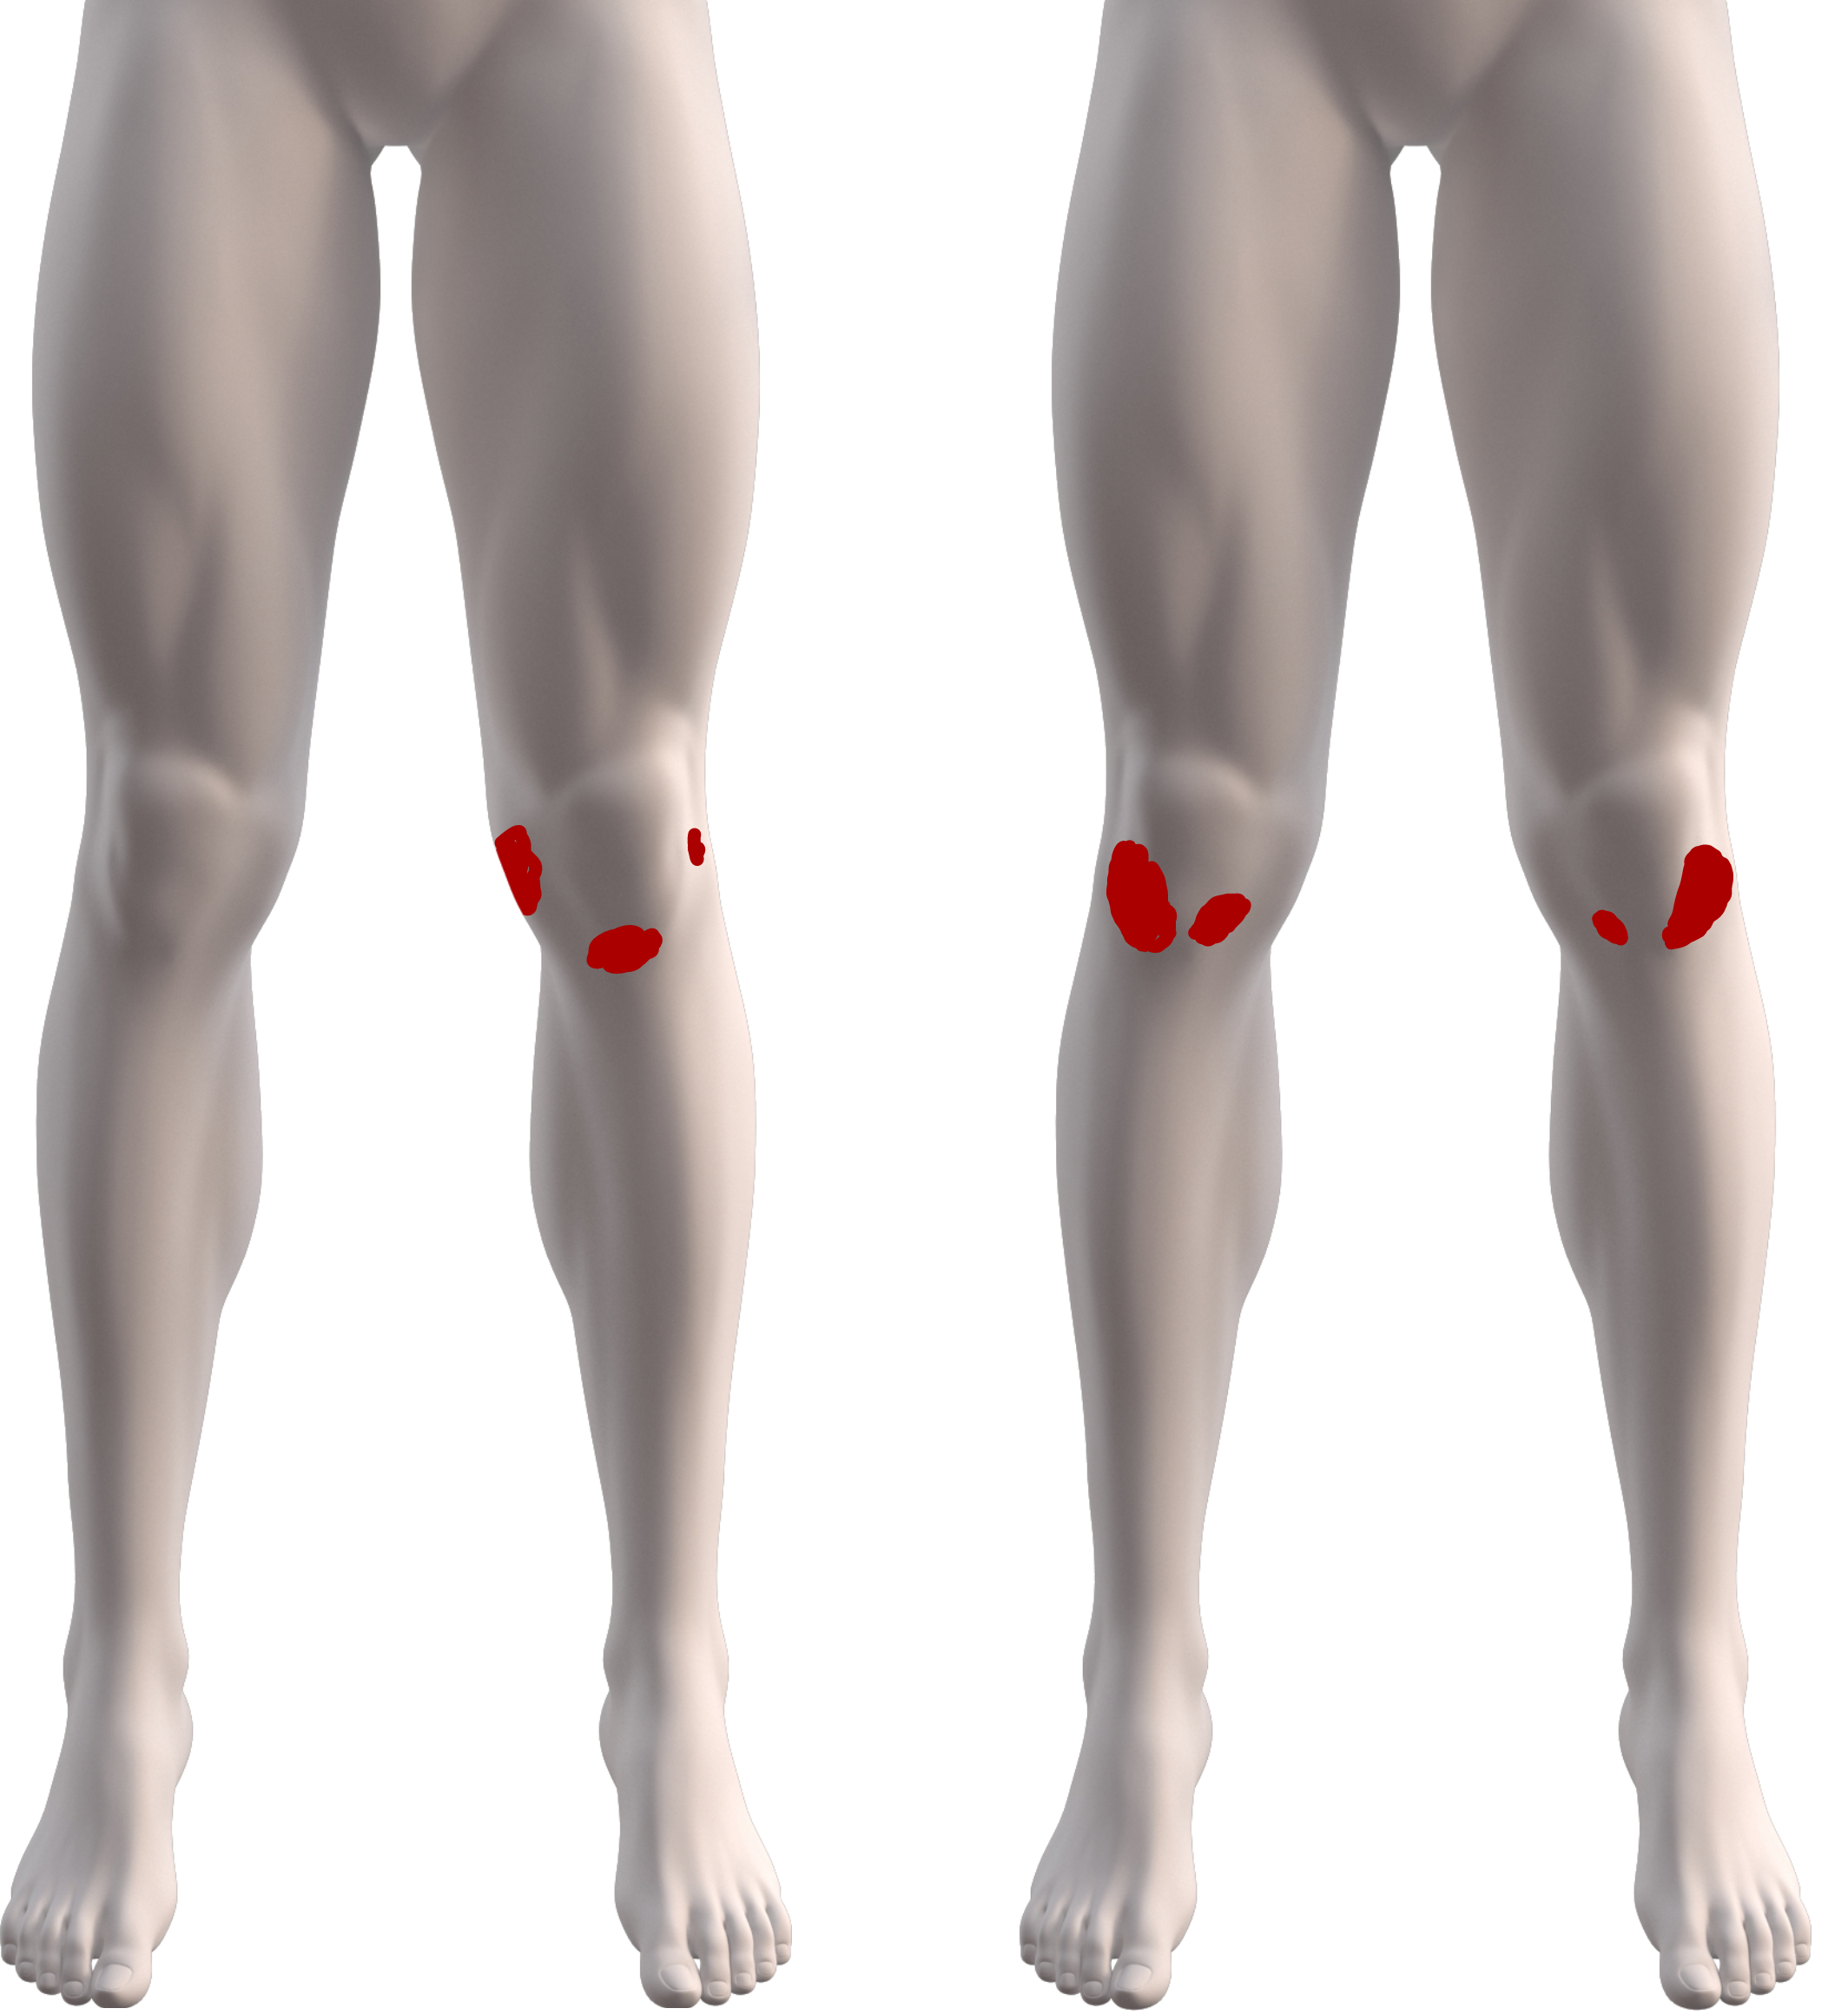
\includegraphics[width=0.35\textwidth]{Figures/twoPainmaps}
\caption{Pain maps from individuals with uni- and bilateral PFP. The red markings indicate the area of pain perceived by the individuals.}
\label{fig:twoPainmaps}
\end{figure}

\noindent
The total number of pain maps available was 217, but only 205 pain maps with associated gender and pain duration, and 197 pain maps with associated gender and pain intensity was available.\\

\noindent
\textbf{Preprocessing} \newline
\noindent
The pain maps were processed in MatLab version R2017b, where the images were resized, since they were collected at different resolutions (screen sizes) and cropped to only include the knees. To create more pain maps is a split body approach used, where pain maps are divided into two knees. Furthermore, pain was mirrored to represent pain on right knees to minimize the variance in the images. By using split body approach it was assumable that the pain duration and pain intensity were identical for both knees if PFP was bilateral. The total number of pain maps with gender and pain duration was 333, and pain maps with gender and pain intensity was 319, of which 15\% was used as test data, and therefore not used to optimize and train the models. \newline
\noindent
The models should classify pain maps according to pain duration or pain intensity divided into intervals. These intervals were created based on the extremes, which were 0 to 12 months and 36 to 300 months for pain duration, and 0 to 4 and 8 to 10 for pain intensity. It was chosen to divide into extremes, since it was assumed that
if the models predicted badly with the extremes, the models would not have a higher predictive value with multiple classifications of the outputs.\\



\noindent
\textbf{Morphology-representation} \newline
\noindent
The original pain maps reflect the morphology of the pain, and do not require further processing than converting the pain maps to a matrix including gender and the output, pain duration or pain intensity. As a result of using the extremes for classifying the number of pain maps decrease to 236 for pain duration, and 196 for pain intensity.\\


\noindent
\textbf{Pain location} \newline
\noindent
The knees are divided into regions based on the underlying anatomical structures, which may have a correlation to pain duration or pain intensity.
The locations are divided into 10 regions, which are inspired by Photographic Knee Pain Map (PKPM). The divisions are designed to categorise location of knee pain for diagnostic and research purposes. PKPM represent both knees that makes it possible to identify unilateral and bilateral pain.\citep{Elson2010} The knee regions are illustrated in fig. \ref{fig:atlas}.

\begin{figure} [H] 
\centering
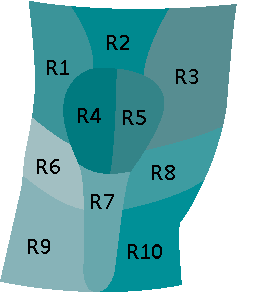
\includegraphics[width=0.35\textwidth]{Figures/atlas}
\caption{The regions of the left (L1-L10) and right (R1-R10) knees, where each knee is split into ten regions.}
\label{fig:atlas}
\end{figure}

\noindent 
There are ten regions, where region 1 and 3 represent the superior lateral and superior medial areas for patella. Region 2 refers to quadriceps tendon. The patella is divided into lateral and medial regions, which are region 4 and 5. Region 6 and 8 are lateral and medial joint line areas. Patella tendon is region 7 and the two last regions, 9 and 10, are tibia lateral and medial.\citep{Elson2010}\\


\noindent
\textbf{Location-representation} \newline
\noindent
To investigate whether the location alone have a correlation to the outputs, a simplified representation of the pain maps was created. The location of the pain was reflected by the use of the defined knee regions (fig. \ref{fig:atlas}), where each region represented a value of 0 (not active) or 1 (active) in a vector.  The values were defined by using a threshold to determine whether a region was considered active in relation the amount of pain. A threshold was required to increase the confidence of an active pain region by avoiding minimal contributions e.g. small pain areas in the associated regions. Simultaneously the threshold should not be too large so that pain areas was excluded. The threshold was decided based on an analysis on five random pain maps, where threshold values of 0, 5, 10 and 15\% was compared. The threshold represent which minimal percentage of pain should be present in a specific region before it is considered active. Based on the analysis a 5\% threshold was chosen. As a result of using the extremes for classification, and adding the threshold value the number of pain maps with pain duration decrease to 223, and number of pain maps with pain intensity decrease to 186.  \\

\noindent
\textbf{Combined-representation} \newline
\noindent
A combination of morphology and location of the pain is created based on components from morphology- and location-representations. The original pain maps are superimposed on the regions, which result in pain pixels reflecting the location with a number from 1 to 10. Before using the representation as input, one-hot encoding approach was used, which made it possible to separate categorical data into binary data \citep{Harris2012}. This means that the 10 values do not have a correlation when analysed in the deep learning model. The number of pain maps with pain duration was 331, and number of pain maps with pain intensity was 317. The number of pain maps increased according to the location-representation, because no threshold was applied in this data-representation. By classifying according to the extremes, the number of pain maps decrease to 234 for pain duration, and 194 for pain intensity.\\

\noindent
\textbf{Nonlinearity in pain maps} \newline
\noindent
Given that PFP is subjective and multifactorial it is unlikely that the pain maps and pain duration or pain intensity are linearly correlated. In order to determine if there was a linear relationship, linear regressions were done on simple features reflecting the size of the pain and number of active pain regions. The linear regressions were made in MatLab, and composed a correlation between number of pain pixels and pain duration, number of pain pixels and pain intensity, number of active pain regions and pain duration, and number of active pain regions and pain intensity.\\


\noindent
\textbf{Deep learning models}\newline
\noindent
Deep learning models were developed on a computer with 4x ‘‘Intel® Core™ i7‘‘ CPUs and one single GPU of type "Geforce GTX 970M", using the programming language Python v3.6.3. Libraries used was Keras with a TensorFlow backend. \newline
\noindent
Multiple deep learning models suitable to the three data representation were created. The models used supervised learning, which is defined as a network learning to classify a given input corresponding to a specific output \citep{Goodfellow2016}. The models classify the input, pain maps and gender, in relation to the determined outputs, pain duration or pain intensity.\newline
\noindent
Two of the models, which managed the morphology-, and the combined morphology and location-representations, were developed using the same model architecture consisting of convolutional- followed by pooling layers and fully connected layers. Convolutional were used because it’s highly classification in images that automatically learn a complex pattern by extracting visual features from the pixel-level content \citep{Acquarelli2017,LeCun1998}. The combination of convolutional and pooling layers performed feature extraction while the classification was made by fully connected layers. \newline
\noindent
The model that classified the location should not process morphology, thus a convolutional layer was not necessary, and thereby only contained fully connected layers. \\


\noindent
\textbf{Optimization of models}\newline
\noindent
Optimization of the three model were done using a validation subset, whereto graphs plotting validation accuracy and loss were compared with training accuracy and loss. This was used to estimate the optimal number of epochs to reduce overfitting the model to the training subset. Further optimization were done using manual search on hyperparameters, from which improvements were based on an average accuracy, sensitivity and specificity gained from 10-fold cross validation.  

%\begin{figure*} [b!]
%\begin{tcolorbox}[colframe=black!30!black, colback=white]
%\centering
%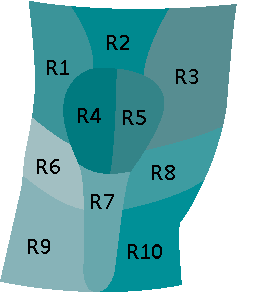
\includegraphics[width=0.2\textwidth]{Figures/atlas}
%\caption{SÅDAN LAVER VI EN BOXER MED ET BILLED}
%\label{fig:atlas1}
%\end{tcolorbox}
%\end{figure*}



%\begin{figure*} [b!]
%\begin{tcolorbox}[colframe=black!30!black, colback=white]
%  \begin{subfigure}[b]{0.45\textwidth}
%    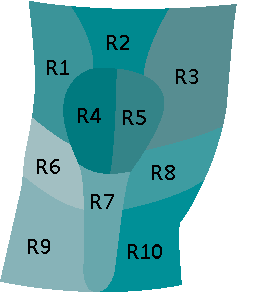
\includegraphics[width=\textwidth]{Figures/atlas}
%    \caption{FUCK JA}
%    \label{fig:f11}
%  \end{subfigure}
%  \hfill
%  \begin{subfigure}[b]{0.45\textwidth}
%    \includegraphics[width=\textwidth]{Figures/twopainmaps}
%    \caption{FUCK NEJ}
%    \label{fig:f22}
%  \end{subfigure}
%  \caption{SÅDAN SÆTTER VI TO BILLEDER I EN}
%\end{tcolorbox}
%\end{figure*}

